As stated in the introduction, finding out the motion of a satellite around a Lagrange point will require us to expand the math that is currently known from IB. 

\subsection{Simple Linear Differential Equations} \label{sec:ode}

Let us imagine that, for some function $f$ with respect to $t$,
\begin{equation}\label{eqn:lde1}
	\frac{d}{dt}f(t) = 4f(t)\text{.}
\end{equation}
In other words, the rate of change of the function $f$ is equal to itself multiplied by four. Let us say we wanted to find what function $f$ is.
While it is not as simple as to integrate this equation, we know that $e^x$ is its own derivative.
We also know that, because of the chain rule, $[e^{kt}]' = ke^{kt}$.
If we substitute $f(t)$ for $e^{kt}$ and let $k = 4$, then Equation \eqref{eqn:lde1} is true.
Therefore, we can state the following \textbf{theorem}; for any equation
\begin{equation}\label{eqn:theory1}
	\frac{d}{dt}f(t) = kf(t)\ :\ f(t) = ce^{kt}
\end{equation}
where $c$ is some initial constant that cannot be expressed from integrating the derivative.
We can verify that this theorem is correct using some algebra and rearranging variables (where $y = f(x)$):
\begin{align*}
	\frac{dy}{dx} &= ky \\
	\frac{1}{y}\, dy &= k\, dx \\
	\int \frac{1}{y}\, dy &= \int k\, dx \\
	\ln y + C &= kx + D \\
	\ln y &= kx + (D - C) \\
	y &= e^{kt} \cdot e^{D - C},\ \text{let}\ c = e^{D - C} \\
	y &= ce^{kt} \text{.}
\end{align*}
Equation \eqref{eqn:lde1} is an example of a differential equation, where a function is defined by its derivatives. Differential equations are very common in physics and will be how our equations of motion will be defined.

\subsection{Eigenvalues and Eigenvectors} \label{sec:eigens}

Imagine that there are two species of ants, $p$ and $q$, whose populations are dependent on each other.
That is to say that both species try to kill the other species while repopulating their own.
We can represent the populations of these two ant species through the following recursive system of equations:
\begin{align*}
	p_{n+1} &=\ \ 4p_n - 2q_n \\
	q_{n+1} &= -3p_n + 5q_n \text{,}
\end{align*}
where each recursive step $n$ represents some interval of time.
Say we knew that, for some initial population of both species, their population would double after the given time interval and we want to know what that initial population would be.
We can determine the initial population by changing our system:
\begin{align*}
	2p_k &=\ \ 4p_k - 2q_k \\
	2q_k &= -3p_k + 5q_k \text{.}
\end{align*}
Then, all that is needed is to solve for $p_k$ and $q_k$:
\begin{equation*}
	\left. \begin{array}{l}
		2p_k =\ \ 4p_k - 2q_k \\
		2q_k = -3p_k + 5q_k
	\end{array} \right \} \implies
	0 = p_k - q_k \implies
	p_k = q_k \text{.}
\end{equation*}
Here, $p_k = q_k$ indicates that any amount of ants is a solution so long as both initial populations have a $1 : 1$ ratio. For example, $p_k = 200$ and $q_k = 200$ is a solution:
\begin{align*}
	2(200) &=\quad \!4(200) - 2(200) = 400 \\
	2(200) &= -3(200) + 5(200) = 400 \text{.}
\end{align*}
In linear algebra, the idea of a linear system with a set of variables being equivalent to scaling said variables is termed an eigenvalue. % more elaboration?
More precisely, an eigenvalue is a numerical constant which represents the factor of which an eigenvector is scaled.
In the case of the ants, the eigenvalue is 2, 
Because linear algebra is beyond the scope of this investigation, we will only explore what is necessary to understand orbital motion.

It is, in fact, possible to determine both the eigenvalues and eigenvectors of most linear systems without knowing either to begin with.
Looking back to our first scaled system, we can generalize it for some eigenvalue $\lambda$ as such:
\begin{align*}
	\lambda p_k &=\ \ 4p_k - 2q_k \\
	\lambda q_k &= -3p_k + 5q_k \text{.}
\end{align*}
The eigenvalues can then be found through substitution and cancelling out the other variables.
\begin{align}
	4p_k - 2q_k &= \lambda q_k \nonumber \\
	(4 - \lambda)p_k &= 2q_k \nonumber \\
	\frac{(4 - k)p_k}{2} &= q_k \nonumber \\
	-3p_k + 5q_k &=\lambda q_k \nonumber \\
	-3p_k &= (\lambda - 5)q_k \nonumber \\
	-3p_k &= (\lambda - 5)\frac{(4 - \lambda)p_k}{2} \nonumber \\
	3\cdot2 &= (5 - \lambda)(4 - \lambda) \nonumber \\
	0 &= (5 - \lambda)(4 - \lambda) - 3\cdot2 \label{eqn:chr-polynomial-ex} \\
	0 &= \lambda^2 - 9\lambda + 14 \nonumber \\
	0 &= (\lambda -2)(\lambda -7) \nonumber
\end{align}
Hence, the eigenvalues are $\lambda_1 = 2$ and $\lambda_2 = 7$.
We can find the respective eigenvector for $\lambda_2$ by doing the same operation for $\lambda_1$.
\begin{equation*}
	\left. \begin{array}{l}
		7p_k =\ \ 4p_k - 2q_k \\
		7q_k = -3p_k + 5q_k
	\end{array} \right \} \implies
	0 = -3p_k - 2q_k \implies
	3p_k = -2q_k \text{.}
\end{equation*}
This gives us an eigenvector of $(-2,3)$.
While a negative amount of ants does not make much sense, these values will be important later for when we want to generalize this system.

From Equation \eqref{eqn:chr-polynomial-ex}, we can generalize the computation of any linear system with 2 variables and 2 equations as:
\begin{equation*}
	0 = (a - \lambda)(d - \lambda) - bc \text{,}
\end{equation*}
where $a,b,c,d$ are the coefficients of the linear system. This computation of solving for eigenvalues can be extrapolated for larger systems involving $n$ variables and $n$ equations.
For a linear system with 3 variables, 3 equations and 9 constants $a, b, \dots, i$:
\begin{equation*}
	0 = (a - \lambda)((e - \lambda)(i - \lambda) - fh) - b(d(i - \lambda) - fg) + c(dh - eg) \text{.}
\end{equation*}
And for 4 variables, 4 equations,and :
\begin{equation*}
	1 = 1 
\end{equation*}
Their solutions are worked through in Appendix \ref{app:eigen}.

\subsection{Systems of Linear Differential Equations} \label{sec:ode-sys}

Now that we have some understanding of what can be done with a linear system, it is time to combine linear systems with calculus.

Now say that we wanted to generalize our system of equations so that we can determine either ant population for some time, $t$.
From what has already been established, this relation would be defined as:
\begin{align*}
	p'(t) &=\ \ 4p(t) - 2q(t) &p(0) = 4\\
	q'(t) &= -3p(t) + 5q(t) &q(0) = 2
\end{align*}
The approach to solving for $p(t)$ and $p(t)$ is not immediately intuitive. Now is a good time to view eigenvalues and eigenvectors in a more abstract manner.
\begin{figure}[H]
	\centering
	\captionsetup[subfigure]{justification=centering}
	\begin{subfigure}[b]{0.4\textwidth}
		\centering
		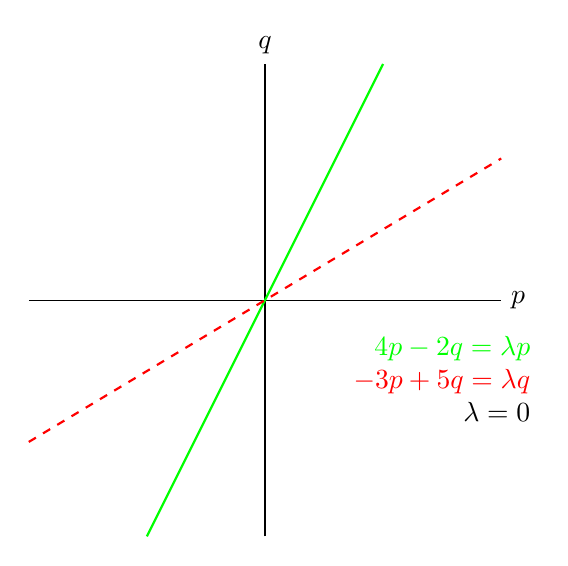
\begin{tikzpicture}
			\draw (-3,0) -- (3,0) node[right] {$p$};
			\draw (0,-3) -- (0,3) node[above] {$q$};
			\draw[thick,green] (-1.5, -3) -- (1.5,3);
			\draw[thick,dashed,red] (-3,-1.8) -- (3,1.8);
			\node at (1,-1) [right,align=right] {$\textcolor{green}{4p - 2q = \lambda p}$ \\
				$\textcolor{red}{-3p + 5q = \lambda q}$ \\
				$\textcolor{black}{\lambda = 0}$};
		\end{tikzpicture}
		\caption{\small Linear system with $\lambda = 0$.}
		\label{fig:sample-eigens0}
	\end{subfigure}
	\quad
	\begin{subfigure}[b]{0.4\textwidth}
		\centering
		\begin{tikzpicture}
			\draw (-3,0) -- (3,0) node[right] {$p$};
			\draw (0,-3) -- (0,3) node[above] {$q$};
			\draw[thick,green] (-2, 3) -- (2,-3);
			\draw[thick,dashed,red] (-2,3) -- (2,-3);
			\filldraw[black] (-1,1.5) circle (1.25pt) node[anchor=east] {$\textcolor{black}{(-2,3)}$};
			\node at (1,-1) [right,align=right] {$\textcolor{green}{4p - 2q = \lambda p}$ \\
				$\textcolor{red}{-3p + 5q = \lambda q}$ \\
				$\textcolor{black}{\lambda = 7}$};
		\end{tikzpicture}
		\caption{\small Linear system with $\lambda = 7$.}
		\label{fig:sample-eigens1}
	\end{subfigure}
	\caption{The linear system defined with regard to $\lambda$ (It is better to think of the graphs as ratios between $p$ and $q$ rather than $q$ as a function of $p$).}
	\label{fig:sample-eigens}
\end{figure}
In Figure \ref{fig:sample-eigens0}, where the $p$ and $q$ are viewed as a set of values, the equations representing the ant species are on different lines with an intersection at $(0,0)$. 
In comparison, in Figure \ref{fig:sample-eigens1}, the equations have converged onto the same line when $\lambda = 7$.
This can be thought of as, for each eigenvalue, $p'(t)$ and $q'(t)$ are transformed onto a function which both share in common.
We will call these `common' functions $x(t)$ and $y(t)$.
The eigenvalues can define these `common' functions as:
\begin{align*}
	x'(t) &= \lambda_1 x(t) \\
	y'(t) &= \lambda_2 y(t) \text{,}
\end{align*}
and are connected back to the functions $p(t)$ and $q(t)$ by the eigenvectors:
\begin{align*}
	p(t) &= (1)x(t) + (-2)y(t) \\
	q(t) &= (1)x(t) + (3)y(t)
\end{align*}
What we have essentially done is factored out a group of functions $x(t)$ and $y(t)$ from the linear system that are much easier to to solve alongside a set of coefficients, the eigenvectors, that relate $x(t)$ and $y(t)$ to $p(t)$ and $q(t)$.
Solving for the `common' functions:
\begin{align*}
	x'(t) &= 2x(t) & x(t) &= c_1e^{2t} \\
	y'(t) &= 7y(t) & y(t) &= c_2e^{7t}
\end{align*}
Then we relate the these back to our original functions:
\begin{align*}
	p(t) &= c_1e^{2t} - 2c_2e^{7t} \\
	q(t) &= c_1e^{2t} + 3c_2e^{7t}
\end{align*}
All that is left is to solve for the given initial conditions:
\begin{align*}
	\left. \begin{array}{l}
		p(0) = 4 = c_1 - 2c_2 \\
		q(0) = 2 = c_1 + 3c_2
	\end{array} \right \} &\implies 2 = -5c_2 \implies -\frac{2}{5} = c_2 \\
	4 = c_1 - 2\left(-\frac{2}{5}\right) &\implies \frac{16}{5} = c_1 \\
	p(t) &= \frac{16}{5}e^{2t} + \frac{4}{5}e^{7t} \\
	q(t) &= \frac{16}{5}e^{2t} - \frac{6}{5}e^{7t}
\end{align*}
This approach to solving equations will be crucial for the next steps involving the equations of motion.
More specifically, this will allow us to separate the dimensions from our equations of motion and determine the appropriate initial velocity given initial coordinates to the proximity of the Lagrange points.